\documentclass[10pt]{article}

\usepackage[cp1251]{inputenc}
\usepackage[T2A]{fontenc}
\usepackage[russian, english]{babel}

\usepackage{amssymb, amsmath, textcomp, tabularx, graphicx}

\newcolumntype{C}{>{\centering\arraybackslash}X}%

\let \eps \varepsilon

\title{Задание 11}
\author{Коновалов Андрей, 074}
\date{}

\begin{document}

\maketitle

\noindent
\begin{tabularx}{\textwidth}{|C|C|C|C|C|C|}
  \hline
  1 & 2 & 3 & 4 & 5 & $\sigma$ \\
  \hline
  &&&&& \\
  \hline
\end{tabularx}

\bigskip

{\bf Задача 1}

Построим ПДКА КМП для языка $L$.

\centerline{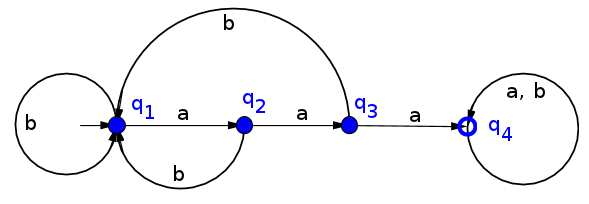
\includegraphics{1.png}}

$M$ будет иметь образующие $\{ 2344, 1114 \}$.
Замыканием этого множества будет $M = \{ 1234, 2344, 4444, 1444, 1144, 1114, 2444, 2244, 2224, 3444, 3344, 3334 \}$.

Отождествим элементы моноида и состояния автомата, по нему построенному, для удобства записи.
Автомат, построенный по моноиду переходов языка $L$ обозначим $A_{M}(L)$.

Автомат $A_{M}(L^{\frac{1}{3}})$ будет иметь такие же состояния, как $A_{M}(L)$, но финальными будут лишь те состояния $x$, для которых $x^3 \in F(A_{M}(L))$.
Рассчитаем $x^3$ для каждого $x \in Q(A_{M}(L))$.

\centerline{
\begin{tabular}{|c|c|c|c|c|c|c|}
  \hline
  $x$      & 1234 & 2344 & 4444 & 1444 & 1144 & 1114 \\
  \hline
  $x^3$    & 1234 & 4444 & 4444 & 1444 & 1144 & 1114 \\
  \hline
  $\in F?$ & +    &      &      & +    & +    & +    \\
  \hline
  \hline
  $x$      & 2444 & 2244 & 2224 & 3444 & 3344 & 3334 \\
  \hline
  $x^3$    & 4444 & 2244 & 2224 & 4444 & 4444 & 3334 \\
  \hline
  $\in F?$ &       & +    & +    &      &      & +    \\
  \hline
\end{tabular}
}

Построим $A_{M}(L^{\frac{1}{3}})$. При его минимизации оказывается, что он уже минимален. Приведем сертификат (разбиение множества состояний на множества k-эквивалентности).
\begin{align*}
  k =& 0: \{ 1234, 1114, 2224, 3334, 1144, 2244, 1444 \}, \{ 2344, 3344, 3444, 2444, 4444 \} \\
  k =& 1: \{ 1234, 2244, 1444, 3334 \}, \{ 1114, 2224, 1144 \}, \{ 2344, 3344, 3444, 2444 \}, \{ 4444 \} \\
  k =& 2: \{ 1234, 2244 \}, \{ 1444 \}, \{3334 \}, \{ 1114 \}, \{ 2224, 1144 \}, \{ 2344 \}, ..., \{ 4444 \} \\
  k =& 3: \{ 1234 \}, ... , \{ 4444 \}
\end{align*}

Сам автомат изображен ниже.

\centerline{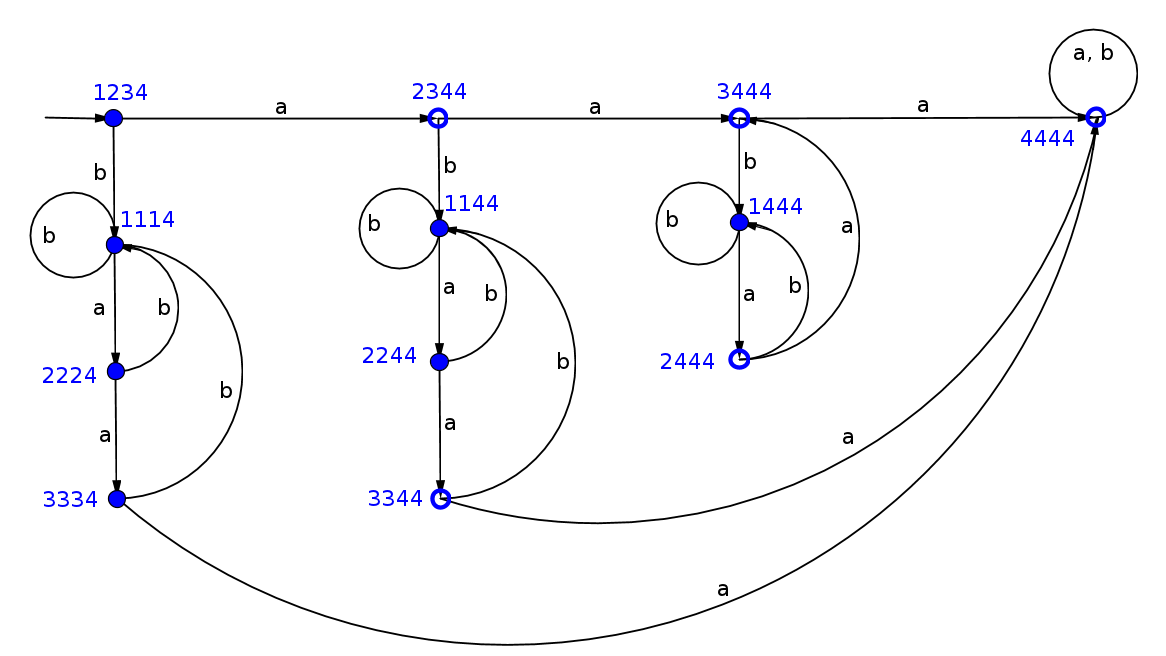
\includegraphics[width=\textwidth]{2.png}}

\medskip

{\bf Задача 2}

{\bf (i)}
Покажем, что $x \sim_A y \Rightarrow x \sim_L y$. Пусть $q_0$ - начальное состояние $A$.
\begin{align*}
  x& \sim_A y \Leftrightarrow \\
  \forall& q \in Q(A) \; \delta(q, x) = \delta(q, y) \Rightarrow \\
  \forall& w \in \Sigma^* \; \delta(q_0, wx) = \delta(q_0, wy) \Leftrightarrow \\
  \forall& w, z \in \Sigma^* \; \delta(q_0, wxz) = \delta(q_0, wyz) \Rightarrow \\
  \forall& w, z \in \Sigma^* \; (wxz, wyz \in L) \vee (wxz, wyz \notin L) \Leftrightarrow \\
  x& \sim_L y
\end{align*}

\smallskip

{\bf (ii)}
Покажем, что $x \sim_{min(A)} y \Leftrightarrow x \sim_L y$.
\begin{align*}
  (x \sim_{min(A)} y \Leftrightarrow& x \sim_L y) \Leftrightarrow \\
  (x \sim_L y \Rightarrow x \sim_{min(A)} y) \, \wedge& \, (x \sim_{min(A)} y \Rightarrow x \sim_L y)
\end{align*}

Из пункта (i) видим, что
\begin{align*}
  x \sim_{min(A)} y \Rightarrow x \sim_L y
\end{align*}

Допустим, что $x \sim_L y$, но $x \nsim_{min(A)} y$, тогда
\begin{align*}
  x& \nsim_{min(A)} y \Rightarrow \\
  \exists& q \in Q(min(A)) \; q_1 = \delta(q, x) \neq \delta(q, y) = q_2
\end{align*}

Поскольку автомат минимальный, то для $q$ существует достигающая цепочка $w$.
\begin{align*}
  x& \sim_L y \Rightarrow \\
  \forall& z \in \Sigma^* (wxz, wyz \in L) \vee (wxz, wyz \notin L) \Rightarrow \\
  \forall& z \in \Sigma^* (\delta(q_1, z), \delta(q_2, z) \in L) \vee (\delta(q_1, z), \delta(q_2, z) \notin L)
\end{align*}

Но это означает, что $q_1$ и $q_2$ - неразличимые, а значит автомат не минимальный.
Противоречие.
Получаем, что $x \sim_L y \Rightarrow x \sim_{min(A)} y$.

\medskip

{\bf Задача 4}

{\bf (i)}
Грамматика, построенная в соответствии с 16.1.6 книги Шеня будет леволинейной.
А значит множество $Left(N)$, которое выводится из $\left\langle LeftN \right\rangle$ является регулярным.

\smallskip

{\bf (ii)}
Обозначим $P = S'$ для удобства. Будем полагать, что $P$ - начальный символ грамматики, поскольку он явно не указан.

В соответствии с 16.1.6 книги Шеня, построим грамматику:
\begin{align*}
  \left\langle LeftP \right\rangle \rightarrow& \; \eps \\
  \left\langle LeftS \right\rangle \rightarrow& \left\langle LeftP \right\rangle \; | \; \left\langle LeftS \right\rangle S a \\
  \left\langle LeftA \right\rangle \rightarrow& \left\langle LeftP \right\rangle S
\end{align*}

Практически очевидно, что из $\left\langle LeftP \right\rangle$ выводится множество $\{ \eps \}$, из $\left\langle LeftA \right\rangle$ - $\{ S \}$, а из $\left\langle LeftS \right\rangle$ - $(Sa)^*$. Автоматы для них строятся тривиально.

\end{document}
